The filter design process is documented in this section, which includes test and optimization. As stated in section \ref{sec:filtervalg} a FIR filter of type I designed by the Kaiser window is wanted.

\subsection{Specifications of the filter} \label{sec:FIRspec} 
By the aim of letting a limited frequency band though the filter - as found in the frequency analysis in chapter \ref{ch9} - the filter is to be designed as a bandpass filter. It is essential to note that the filter to be designed in this project is not an adaptive filter, meaning that the filter specifications will be chosen on behalf of a specific signal including a known noise signal. During final tests the filter is adapted to other signals only by chancing the specifications for the cut off frequencies. \\ \\
This filter is determined to remove noise in the form of clapping hands from a signal representing a low E note. \\
Due to the frequency analysis of single tones described in section \ref{sec:single} the energy in the signal is located within a frequency band from 75 Hz to 1000 Hz.  
By letting the cut off frequencies of the filter be respectively 75 Hz and 1000 Hz, this makes the passband of the filter. Note that the cut off frequencies is given in $[Hz]$ instead of $[rad./sec.]$. To convert between the two the frequencies has to be relative to the sampling frequency $f_s$ such that $f_s = 2\pi$. Thus the normalized transition frequency $f_t$ is defined relatively to the sampling frequency as
\begin{align}
f_t = \frac{\textit{Cut-off frequency}}{\textit{Sampling frequency}}
\end{align}
By the frequency analysis of the specific noise showed by figure \ref{fig:clapping} it is seen that the frequencies of the noise are completely adjacent to the desired passband which verifies the need narrow the  transition band. The narrower transitionband the higher order of filter is need which gives more computer computations. \\  

The peak approximation error $\delta_1$is determined as $\delta_1=0.01$. Further, the maximum allowed width of the transition band is determined by another $\delta_2 = 0.5$ given in $[Hz]$. This gives a transition width at $1 [Hz]$ for each transitionband, normalized this gives $\Delta f_t = \frac{1 }{f_s} \approx 2.26 \cdot 10^{-5}$.\\
The magnitude response of the ideal filter is sketched in figure \ref{fig:spec_Hd}, along with the boundaries for the real filter, provided by the defined specifications.      

\begin{figure}[H]
\centering
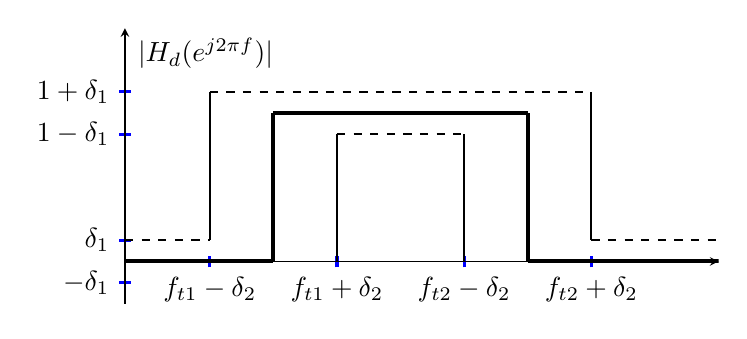
\begin{tikzpicture}[scale=1]
\begin{axis}[every tick/.style={blue, very thick}, 
scale=1.1,
unit vector ratio*=1 1 1,
axis lines = middle,
xtick={2,5,8,11},
xticklabels={$f_{t1}-\delta_2$,$f_{t1}+\delta_2$,$f_{t2}-\delta_2$,$f_{t2}+\delta_2$},
ytick={-0.5,0.5,3,4},
yticklabels={$-\delta_1$,$\delta_1$,$1-\delta_1$,$1+\delta_1$},
xmin=0,
xmax=14,
ymin=-1,
ymax=5.5]
\node at (axis cs:1.9,4.9) {$|H_d(e^{j 2\pi f})|$};
\draw[line width=0.5mm](axis cs:0,0)--(axis cs:3.5,0);
\draw[line width=0.5mm](axis cs:3.5,0)--(axis cs:3.5,3.5);
\draw[line width=0.5mm](axis cs:3.5,3.5)--(axis cs:9.5,3.5);
\draw[line width=0.5mm](axis cs:9.5,3.5)--(axis cs:9.5,0);
\draw[line width=0.5mm](axis cs:9.5,0)--(axis cs:14,0);
\draw[line width=0.25mm, dashed](axis cs:0,0.5)--(axis cs:2,0.5);
\draw[line width=0.25mm, dashed](axis cs:11,0.5)--(axis cs:14,0.5);
\draw[line width=0.25mm, dashed](axis cs:5,3)--(axis cs:8,3);
\draw[line width=0.25mm, dashed](axis cs:2,4)--(axis cs:11,4);
\draw[line width=0.25mm](axis cs:2,0.5)--(axis cs:2,4);
\draw[line width=0.25mm](axis cs:5,0)--(axis cs:5,3);
\draw[line width=0.25mm](axis cs:8,0)--(axis cs:8,3);
\draw[line width=0.25mm](axis cs:11,4)--(axis cs:11,0.5);
%\draw[line width=0.5mm](axis cs:4,0.5)--(axis cs:7,0.5);
%\node at (axis cs:1,1.5) {Passband};
%\node at (axis cs:3,1.5) {Transition};
%\node at (axis cs:5.0,1.5) {Stopband};
\end{axis}
\end{tikzpicture}
\caption{Ideal magnitude response of filter within the boundaries for the amplitude response of the final filter, given by the defined specifications.}
\label{fig:spec_Hd}
\end{figure}

\subsection{Implementation of the filter}
The implementation of the filter basically follows algorithm \ref{alg:FIR}. The ideal impulse response is defined as the inverse Fourier transformation of the ideal filter specified on figure \ref{fig:spec_Hd}. For derivation of the ideal impulse response of a bandpass filter consult appendix \ref{appC}. Figure \ref{fig:freq_filt1} illustrates a plot of the amplitude response corresponding to the filter in the frequency domain. At \ref{fig:freq_filt2} illustrate a close up view of the left transition band, showing the ripples at in stop- and passband  the boundaries from the specifications are marked by the green lines. It is seen that the specifications are fulfilled, with only one minimal exceeding of the limit.        
\begin{figure}[h]
\centering
\begin{subfigure}{0.49\textwidth}
\centering
\includegraphics[width=\textwidth]{figures/filtertest/freq_response1.pdf}
\caption{}
\label{fig:freq_filt1}
\end{subfigure}
\begin{subfigure}{0.49\textwidth}
\centering
\includegraphics[width=\textwidth]{figures/filtertest/freq_response2.pdf}
\caption{}
\label{fig:freq_filt2}
\end{subfigure}
\caption{(a) Amplitude response of filter. (b) Close up amplitude response of filter, showing top and bottom of one transitionband.}
\label{fig:freq_filt}
\end{figure}


\begin{algorithm}[H]
\caption{Compute type I FIR filter}
\label{alg:FIR}
\begin{algorithmic}[1] 
\State $f_s= 44100$ \Comment {Sampling frequency}
\State $f_{t1} = 75/f_s$ \Comment {Transition frequency $1$}
\State $f_{t2} = 1000/f_s$ \Comment {Transition frequency $2$}
\State $\delta_1 = 0.01$  \Comment {Max. amplitude error }
\State $\delta_2 = 0.5 $ 
\State $\Delta f_t = 2 \cdot \delta_2 / f_s$  \Comment {Transition width}
\\
\State $A=-20\log_{10}(\delta_1)$ \Comment{$21 \leq A \leq 50$}
\State $\beta = 0.5824(A-21)^{0.4} + 0.07886(A-21)$ \Comment {Shape parameter}
\State $M = (A-8)/(2.285 \cdot \Delta f_t  2\pi)$ \Comment {Filter order, round to upper even int.}
\State $N = M+1$ \Comment {Lenght of filter}
\\
\Procedure{Compute ideal impulse response}{$h_d$}
    \For {each integer $i$ in $h_d$}
        \If {$i == \frac{M}{2}$}
        		\State $h_d[i] = 2(f_{t2} - f_{t1})$
        	\Else 
        		\State  $h_d[i] = \frac{1}{ (\pi (i - \frac{M}{2}))}(\sin(f_{t2} 2 \pi (i - \frac{M}{2})) - (\sin(f_{t1} 2 \pi (i - \frac{M}{2}))))$ 
        	\EndIf 
	\EndFor
	\State Return $h_d$
\EndProcedure
\\
\Procedure{Compute kaiser window}{$w$}
	\For {each integer $i$ in length of $N$}
		\For {each integer $j$ in length of $M$}
			\State $ sum_n = + \ (\frac{1}{j!})^2 \left( \left( \frac{\beta}{2} \sqrt{\left(1 - \left( \frac{2*i}{N-1}\right) - 1\right)^2}\right)^{2j}\right)$
			\State $ sum_d = + \ (\frac{1}{j!})^2 \left( \frac{\beta}{2}\right)^{j2}$
		\EndFor
		\State $w[i]=\frac{sum_n}{sum_d}$
	\EndFor
	\State Return $w$
\EndProcedure
\\
\Procedure{Compute frequency response}{$H$}
	\State $h = h_d \cdot w$ \Comment{Windowed impulse response}
	\State $H = fft(h)$ \Comment {Fourier transformation of impulse response}
	\State Return $H$
\EndProcedure

\end{algorithmic}
\end{algorithm}

\subsection{Validation of the filter}
The implemented filter is tested according to the test specifications described in section \ref{sec:testspec}. Figure \ref{fig:SIGNAL} show the frequency spectrum of the single low E note with additive noise in form of a beat of hands clapping. Figure \ref{fig:filt_SIGNAL} show the filtered signal. Note that the frequency spectrum are only showed from 0 to approximately 2200 $[Hz]$.  

\begin{figure}[H]
\centering
\begin{subfigure}{0.49\textwidth}
\centering
\includegraphics[width=\textwidth]{figures/filtertest/SIGNAL.pdf}
\caption{}
\label{fig:SIGNAL}
\end{subfigure}
\begin{subfigure}{0.49\textwidth}
\centering
\includegraphics[width=\textwidth]{figures/filtertest/filt_SIGNAL.pdf}
\caption{}
\label{fig:filt_SIGNAL}
\end{subfigure}
\caption{(a) Frequency spectrum of signal with noise (b) frequency spectrum of filtered signal}
\label{fig:test_res}
\end{figure}
As described in the specifications the filter is designed to remove all frequencies outside the frequency band from 75 Hz to 1000 Hz. It is seen by the figures that frequencies outside the passband appears to be zero and that the amplitude of the remaining frequencies are the same. \\
By this the designed filter of order 98294 fulfil the specifications.\\
However, by comparing the filtered signal with the pure music signal, cp. figure \ref{fig:single_low}, it seen that noise occurs in between the significant frequencies that lays in the passband. To remove this noise a multiple bandpass filter is required. \\
On behalf of this test it is assumed that by changing the cut off frequencies the filter can be modified to fit other music signals.  